% !Mode:: "TeX:UTF-8"

\documentclass[proposal]{zjutreport}
\usepackage{url}
\graphicspath{{figures/}}  % 定义所有的eps文件在 figures 子目录下
\begin{document}           % 开始全文

%论文题目:{中文}
\zjuttitle{基于内存数据库的大数据应用系统的设计与实现}
%作者:{中文姓名}{学号}
\zjutauthor{陈佳鹏}{200926630503}
%指导教师:{导师中文名}
\zjutmentor{陈~~~~波}
%个人信息:{毕业年份}{专业名称}
\zjutinfo{2013}{软件工程}
%学院信息:{学院中文}
\zjutcollege{计算机科学与技术学院}
%日期:{提交日期}
\zjutdate{2013年03月}

\input{preface/cover}      % 封面

\frontmatter

\pagenumbering{Roman}
\begingroup % 在组内的chapter不换行
\let\clearpage\relax % chapter之后不换页

%%%%%%%%%% 标题 %%%%%%%%%%
\titleformat{\chapter}[block]{\sihao\heiti\filcenter\bfseries}{\CJKnumber{\thechapter}}{1ex}{}{} % 标题居中,黑体三号
\chapter*{基于内存数据库的大数据应用系统的设计与实现}
\titleformat{\chapter}[block]{\xiaosi\heiti}{\CJKnumber{\thechapter}、}{1ex}{}{} % 恢复标题居左,黑体四号

%%%%%%%%%% 正文 %%%%%%%%%%
\mainmatter
\chapter{选题的背景与意义}
\section{研究开发的目的}
1969年,埃德加•弗兰克•科德(Edgar Frank Codd)发表了一篇划时代的论文,首次提出关系数据模型的概念。但可惜的是,刊登论文的“IBM Research Report”只是IBM公司的内部刊物,因此论文反响平平。1970年,他再次在刊物《Communication of the ACM》上发表了题为“A Relational Model of Data for Large Shared Data banks”(大型共享数据库的关系模型)的论文,终于引起了大家的关注。

科德所提出的关系数据模型的概念成为了现今关系型数据库的基础。当时的关系型数据库由于硬件性能低劣、处理速度过慢而迟迟没有得到实际应用。但之后随着硬件性能的提升,加之使用简单、性能优越等优点,关系型数据库得到了广泛的应用。

但是现如今随着互联网的不断发展,各种类型的应用层出不穷,所以导致在这个云计算的时代,对技术提出了更多的需求,传统关系型数据库面临很多问题,主要体现在下面这四个方面:
\begin{enumerate}[label=(\arabic*)]
\item{低延迟的读写速度:应用快速地反应能极大地提升用户的满意度}
\item{支撑海量的数据和流量:对于搜索这样大型应用而言,需要利用PB级别的数据和能应对百万级的流量}
\item{大规模集群的管理:系统管理员希望分布式应用能更简单的部署和管理}
\item{庞大运营成本的考量:IT经理们希望在硬件成本、软件成本和人力成本能够有大幅度地降低}
\end{enumerate}

虽然关系型数据库已经在业界的数据存储方面占据不可动摇的地位,但是由于其天生的几个限制,使其很难满足下面的这几个需求:
\begin{enumerate}[label=(\arabic*)]
\item{扩展困难:当需要表与表之间Join操作时,数据库就不能很好的进行扩展}
\item{读写速度慢:当数据量达到较大规模的时候,很容易发生死锁的问题,直接导致读写速度急剧下降的问题}
\item{成本高:企业级数据库的License价格惊人,且随着系统的规模而不断上升}
\item{有限的支撑容量:现有关系型解决方案还无法支撑Google这样海量的数据存储}
\end{enumerate}

而因此思想诞生的内存数据库(MMDB)对数据访问读取有着很高的效率,对于一些需要
在严格要求的时间段内完成事务请求
的实时应用系统,和需要支持大量并发访问的高性能事务处理平台来而言,它都是一个很不错的选择。在实际的应用中,经常会出现这样一种情况:不能相互访问其内置实时数据库,使得很多信息冗余于各系统中。为了避免这种问题,必须合理规划管理实时数据库的数据。

\section{研究现状}
目前,大数据时代推动了内存数据库的发展,国内外相关人员经过长年的研究,设计并实现了多种内存数据库的
模型及商用或开源的产品。商用MDB的代表产品有AltiBase、Timesten,SAP HANA等,开源
产品主要有FastDB、SQLite、Redis等,下文对比较热门的Timesten、SAP HANA[8]以及本课题所需的redis做一个简单的介绍。

\subsection{Oracle TimesTen}
Oracle TimesTen内存数据库是一个功能全面的关系型内存数据库,旨在通过在应用层的运行,加速处理响应时间和关键任务型应用所需的高吞吐量。从某种角度上来看,TimesTen也是一种Cache机制,是磁盘数据库的‘Cache’,通过物理内存中的数据存储区的直接操作,减少了到磁盘间的I/O交互。TimesTen中的这个Ten据说就是指速度能达到基于磁盘的RDBMS10倍。

\subsection{SAP HANA}
SAP HANA是一款面向数据源的、灵活、多用途的内存应用设备,整合了基于硬件优化的SAP软件模块,通过SAP主要硬件合作伙伴提供给客户。SAP HANA提供灵活、节约、高效、实时的方法管理海量数据。利用HANA,企业可以不必运行多个数据仓库、运营和分析系统,从而削减相关的硬件和维护成本。SAPHANA将在内存技术基础上,为新的创新应用程序奠定技术基础,支持更高效的业务应用程序,如:计划、预测、运营绩效和模拟解决方案。

\subsection{Redis}
Redis是一个高性能的key-value存储系统。和Memcached类似,它支持存储的value类型相对更多,包括string(字符串)、list(链表)、set(集合)和zset(有序集合)。这些数据类型都支持push/pop、add/remove及取交集并集和差集及更丰富的操作,而且这些操作都是原子性的。在此基础上,redis支持各种不同方式的排序。与memcached一样,为了保证效率,数据都是缓存在内存中。区别的是redis会周期性的把更新的数据写入磁盘或者把修改操作写入追加的记录文件,并且在此基础上实现了master-slave(主从)同步。

\chapter{研究开发的目标、基本内容,技术关键}
\section{研究目标}
通过阅读源码和相关资料来了解Redis的工作原理,从数据结构到服务器构造在内的相关知识,并应用于实际的大数据中。
本课题的研究目标定位于利用Redis基本架构,从而实现一个简单的大数据应用系统。

\section{基本内容}
本课题研究的基本内容可以分成三部分:
\begin{enumerate}[label=(\arabic*)]
\item{了解Redis的工作原理,包括内部数据结构(动态字符串、双端列表、字典、跳跃表),内存映射数据结构(整数集合、压缩列表),数据类型(对象处理机制、字符串、哈希表、列表、集合、有序集),功能的实现(事务、订阅与发布、慢查询日志),内部运作机制(数据库、rdb、aof、事件、服务器与客户端)
}
\item{支持SQL语言的存储引擎设计:支持基础的查询修改等SQL}
\item{设计开发图形化的性能测试工具:能准确明显得反应出内存数据库和磁盘数据库之间性能的差距}
\end{enumerate}

\section{技术关键和难点}
\begin{enumerate}[label=(\arabic*)]
\item{了解Redis的工作原理,包括这些方面:内存所使用的数据结构和算法、目前正在使用的两种内存映射数据结构、所使用的对象系统,字符串、哈希表、列表、集合和有序集类型的底层实现,一些辅助性的功能,比如慢查询,以及一些和数据库无关的功能,比如订阅与发布,需要这些功能的底层实现。此外,如何表示一个数据库?数据库操作是如何实现的?
如何进行持久化?RDB模式和AOF模式有什么区别?
如何处理输入命令?它又是如何将输出返回给客户端的?
服务器如何初始化?传入服务器的命令又是以什么方法执行的?}
\item{支持SQL语言的存储引擎设计:如何支持最基本的SQL语句,包括select,update等}
\item{图形化性能测试工具的开发:如何设计测试工具,能直观明显的反应内存数据库和磁盘数据库之间性能的差距}
\end{enumerate}

\newpage

\chapter{研究开发的方法、技术路线和步骤}
\begin{enumerate}[label=(\arabic*)]
\item{Redis架构
\begin{figure}[htbp]
\centering
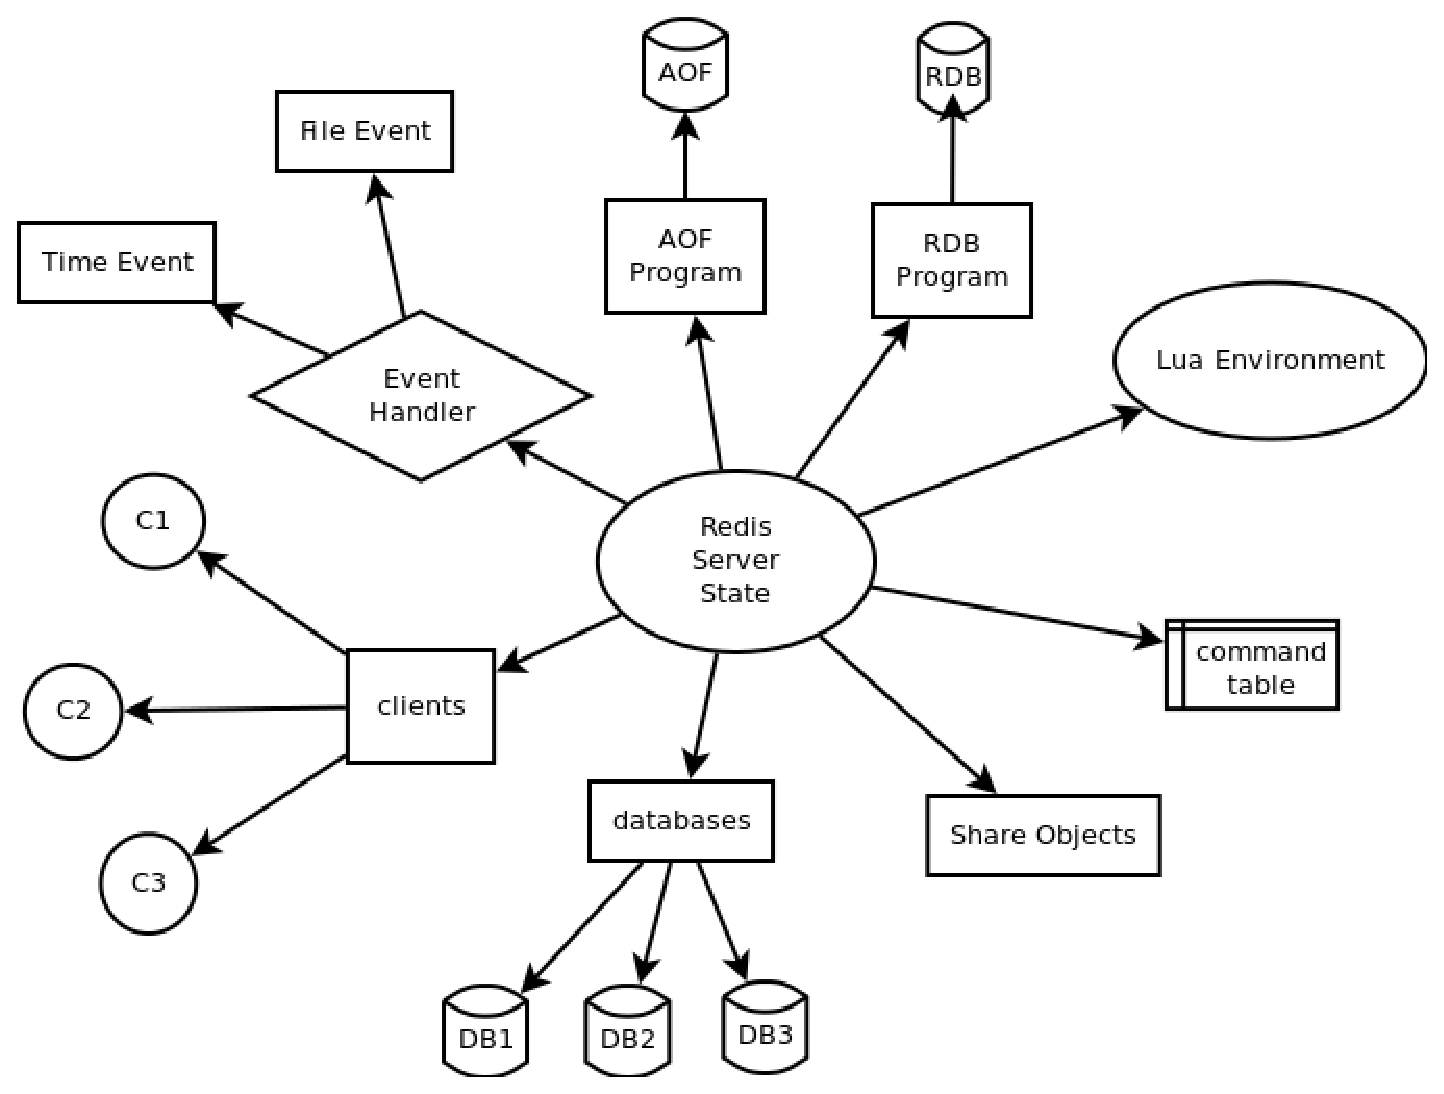
\includegraphics[width=0.7\textwidth]{redis-server}
\caption{Redis架构}\label{fig:redis-server}
\vspace{\baselineskip}
\end{figure}
}%end Redis架构

\item{Redis运行流程[22]

\begin{enumerate}[label=\arabic*.]
\item{服务器初始化:从启动Redis服务器,到服务器可以接受外来客户端的网络连接这段时间,Redis需要执行一系列初始化操作。整个初始化过程可以分为六个步骤:
\begin{enumerate}[label=\Roman{*}.]
\item{初始化服务器全局状态}
\item{载入配置文件}
\item{创建daemon进程}
\item{初始化服务器功能模块}
\item{载入数据}
\item{开始事件循环}
\end{enumerate}
}

\item{当一个客户端通过套接字函数connect到服务器时,服务器执行以下步骤:
\begin{enumerate}[label=\Roman{*}.]
\item{服务器通过文件事件无阻塞地accept客户端连接,并返回一个套接字描述符fd}
\item{服务器为fd创建一个对应的redish/redisClient结构实例,并将该实例加入到服务器的已连接客户端的链表中}
\item{服务器在事件处理器为该fd关联读文件事件}
\end{enumerate}
}

\item{
当客户端连上服务器之后,客户端就可以向服务器发送命令请求了。
从客户端发送命令请求,到命令被服务器处理、并将结果返回客户端,整个过程有以下步骤:
\begin{enumerate}[label=\Roman{*}.]
\item{客户端通过套接字向服务器传送命令协议数据}
\item{服务器通过读事件来处理传入数据,并将数据保存在客户端对应redisClient结构的查询缓存中}
\item{服务器在事件处理器为该fd关联读文件事件}
\item{根据客户端查询缓存中的内容,程序从命令表中查找相应命令的实现函数}
\item{程序执行命令的实现函数,修改服务器的全局状态server变量,并将命令的执行结果保存到客户端redisClient结构的回复缓存中,然后为该客户端的fd关联写事件}
\item{当客户端fd的写事件就绪时,将回复缓存中的命令结果传回给客户端}
\end{enumerate}
}
\end{enumerate}
}
\item{编程语言:Python\\
Python现在是最流行的动态编程语言之一,紧接着是Perl,Tcl,PHP和最近的Ruby。虽然它经常被看做是“脚本语言”,但实际上它是和List或者Smalltalk类似写法的通用编程语言。今天,python被用在很多地方,从使用完就扔的脚本到提供24x7不间断服务的大型web服务。它还用在GUI和数据库编程,客户端和服务端web编程,程序测试。
作为一种即译式的,互动的,面向对象的语言,它包含了异常处理,动态资料形态,高层次的动态结构,和类别的使用。Python语法简单,但是功能出奇的强大。其表达式语法优美易读。并包含了其他优秀脚本语言的一些特点:解释的,面向对象,内置的高级数据结构,支持包以及模块,多平台,可扩展。
}
\end{enumerate}

\newpage

\chapter{研究工作总体安排与时间进度}
\begin{table}[htbp]
\caption{工作总体安排与时间进度}\label{tab:table1}
\vspace{0.5em}
\begin{center}
{\wuhao
\begin{tabular}{|c|c|c|}
\hline
任务序号 & 起止时间 & 阶段任务要点\\ \hline
1 & 2013.1.11~-~2013.2.20 & 了解课题相关内容,查找中、英文资料\\ \hline
2 & 2013.2.21~-~2013.3.8 & 查阅文献资料,完成文献综述、开题报告和外文翻译\\ \hline
3 & 2013.3.9~-~2013.3.25 & 阅读Redis源代码,分析其架构\\ \hline
4 & 2013.3.26~-~2013.4.1 & 系统详细设计\\ \hline
5 & 2013.4.2~-~2013.4.24 & 编码\\ \hline
6 & 2013.4.25~-~2013.4.30 & 系统测试\\ \hline
7 & 2013.5.1~-~2013.5.15 & 整理资料,完成论文\\ \hline
\end{tabular}}
\end{center}
\vspace{\baselineskip}
\end{table}

\backmatter
\endgroup % 组结束
%%%%%%%%%% 参考文献 %%%%%%%%%%
\clearpage % 显式换页,使书签定位准确
\bibliography{references/reference}
\nocite{*}                                   % 若将此命令屏蔽掉,则未引用的文献不会出现在文后的参考文献中。

%%%%%%%%%% 附录 %%%%%%%%%%
%\appendix
%\include{appendix/appendix}            % 附录

\end{document}                                  % 结束全文
